\documentclass{beamer}
\usepackage[utf8x]{inputenc}
\usepackage[ngerman]{babel}
\usepackage{amsmath}
\usepackage{amsfonts}
\usepackage{amssymb}
\usepackage{graphicx}
\usepackage{hyperref}
\usepackage{listings}
\lstset{literate=%
{Ö}{{\"O}}1
{Ä}{{\"A}}1
{Ü}{{\"U}}1
{ß}{{\ss}}2
{ü}{{\"u}}1
{ä}{{\"a}}1
{ö}{{\"o}}1
}

\lstset{language=C}

\author{Johannes Hackel \and Falco Prescher}
\title{OpenCL}

\usetheme{Ilmenau}
\useoutertheme{infolines}
\usecolortheme{rose}

\begin{document}

\begin{frame}
\titlepage
\end{frame}

\begin{frame}
\frametitle{Gliederung}
\tableofcontents
\end{frame}

\section{Was ist OpenCL?}
\begin{frame}[fragile]
\frametitle{Was ist OpenCL?}
%\url{http://en.wikipedia.org/wiki/OpenCL}
\end{frame}
\subsection{Geschichte}
\begin{frame}[fragile]
\frametitle{Geschichte}
%\url{http://en.wikipedia.org/wiki/OpenCL#History}
\end{frame}
\subsection{Unterstütze Geräte/Treiber}
\begin{frame}[fragile]
\frametitle{Unterstütze Geräte/Treiber}
%\url{http://en.wikipedia.org/wiki/OpenCL#OpenCL-conformant_products}
\end{frame}

\section{Aufbau GPUs}
\begin{frame}[fragile]
\frametitle{Aufbau GPUs}
\begin{itemize}
\item Grafikprozessor besteht aus Recheneinheiten, ähnlich CPU:
\item Ausführung Operationen der Arithmetik, Decodierung und Datentransfer
\item Verarbeitung paralleler Prozesse (zB. mathematischer Operationen) bei konstanter Taktrate
\item Durch breiten Datenbus mit Speichereinheit verbunden, großer Datendurchsatz
\item Verarbeitung vieler Daten gleichzeitig:
\item graphische, dreidimensionale Objekte, Beleuchtung, Farben und Texturen
\item Auswertung wissenschaftliche Daten
\item Simulation komplexer physikalischer Systeme (zB. viele kleine Teilchen)
\end{itemize}
\end{frame}

\begin{frame}[fragile]
\begin{figure}
\begin{center}
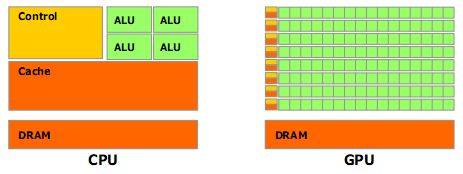
\includegraphics[width=10cm]{cpu_gpu.png}
\end{center}
\end{figure}
\end{frame}

\section{Die OpenCL}
\subsection{Kernel}
\begin{frame}[fragile]
\frametitle{Die OpenCL}
\framesubtitle{Kernel}
\begin{lstlisting}
float Sum(float x, float y)
{
 return(x + y);
}

__kernel void Calculate(__global float* input,
 __global float* output)
{
 
}
\end{lstlisting}
\end{frame}

\subsection{Speicherbereiche}
\begin{frame}[fragile]
\frametitle{Speicherbereiche}
\begin{center}
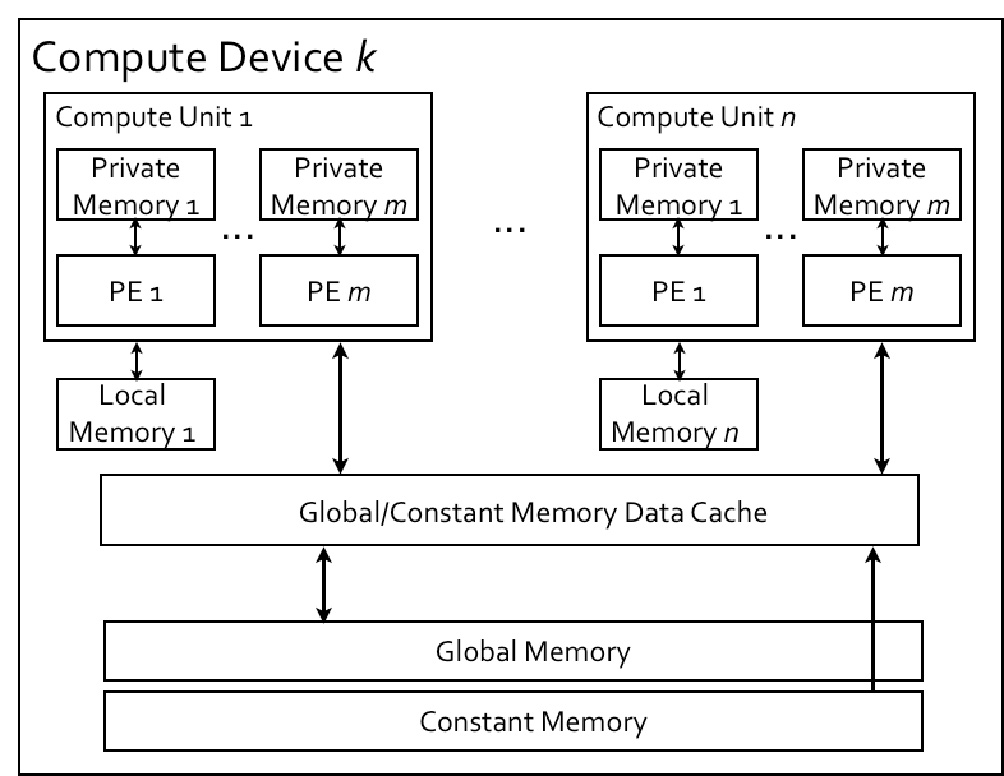
\includegraphics[width=10cm]{opencl_memory.jpg}
\end{center}
\end{frame}

\begin{frame}[fragile]
\frametitle{Speicherbereiche}
privater Speicher:
\begin{itemize}
\item \_\_private
\item Variablen die in einer Funktion deklariert wurden und Funktionsargumente
\item nur in dieser Funktion zugänglich
\item existieren nur für die jeweilige Kernel-Instanz
\end{itemize}
lokaler Speicher:
\begin{itemize}
\item \_\_local
\item werden von allen Kernel-Instanzen in einer Arbeitsgruppe gemeinsam genutzt
\item jede Arbeitsgruppe besitzt eigene Kopie 
\end{itemize}
\end{frame}

\begin{frame}[fragile]
\frametitle{Speicherbereiche}
globaler Speicher:
\begin{itemize}
\item \_\_global
\item Zugriff von Host und Client möglich
\item üblicherweise ein Zeiger auf Speicherbereich
\item alle Kernel-Instanzen greifen auf die selben Daten zu
\end{itemize}
Konstantenspeicher:
\begin{itemize}
\item \_\_constant
\item nur lesbar
\item kann in lokalen Speicher liegen
\end{itemize}
\end{frame}

\section{Quellen}
\begin{frame}[fragile]
\frametitle{Quellen}
\begin{itemize}
\item \url{http://www.khronos.org/}
\item \url{hexagon.fi.tartu.ee/~manuel/teaching/gpu.pdf}
\item \url{http://www.zdnet.de/wp-content/uploads/legacy_images/news/201004/aws-gpu-v6.png}
\item \url{http://developer.amd.com/Resources/documentation/articles/PublishingImages/opencl_figure5.jpg}
\end{itemize}
\end{frame}
\end{document}